\documentclass[twocolumn]{article}
\usepackage[colorlinks=true]{hyperref}
\usepackage{graphicx}
\begin{document}
%setting the title
\title{Homework 1: Implementation of Robot Planning and Controls}
%setting the author
\author{Ivan D. Jimenez}
\date{January 15, 2014}
\maketitle

In this iteration of the course I wish to delve further into the implementation of planning algorithms. Since there have been several algorithms tested and implemented in this class, I believe it is time to put all our planning experience into a single useful application. Given the complexity of the system we are dealing with, such application will pose as much a software engineering challenge as a planning challenge.

The first challenge we are facing is creating an application that can handle an constantly updating stream of data to maintain a goal-directed plan. Even a light glance at such a problem indicates a necessary use of threading. Still dealing with a updating data is only half of the challenge. After all, we are facing a constant duality between the translation movement that will require 2-D planning and arm movement that will require 5-D and 3-D planning.

For two dimensional planning we can use optimal algorithm's that may only work in a reasonable time on 2-D space. The most commonly used one is A* for its reasonably fast search and optimization of the path. Since we are also dealing with a constant stream of data, it would be wise to implement and study D*, a variant of A* that utilizes new data as it becomes available. 

At the same time, we need to make a path for the arm to reach its three dimensional position. This, however, is not a trivial task given the large number of joints in the Kuka Youbot. To do this we will have to perform a search in the 5-D joint space of the arm and the 3-D space that the robot actually interacts with. 

To ensure that we solve the problem or at least give a thorough inspection to all possible solutions, we can implement a variety of algorithms used for such complex planning. These are all based on Rapidly-Exploring Random Trees(RRTs). From the original RRT we have evolved in the way we utilize this data structure and algorithm to explore high-dimensional spaces for paths.

There have been several improvements to this basic algorithm that significantly improve its speed. From last year, simply implementing it using a k-d tree instead of a basic array as a data structure to hold the tree would provide a significant speed boost. However, when searching for optimal speeds in finding a good path simply generating a random path and trimming it may not be sufficient. 

Bidirectional RRTs are the beginning of optimization options. By placing an RRTs that search each other based at the start and end points, we increase the search speed significantly. There have also been improvements on optimality and speed by combining this technique and dynamic programming to produce RRT* and RRT#: newer versions of the algorithm that promise an asymptotic optimal path. 

Thus, the task of implementing usable planning application remains daunting. We will have to create an application that uses the map generated by the visual sensors to generate the commands that the robot has to use to get from starting point to end point. 

\begin{figure}[ht!]
\centering
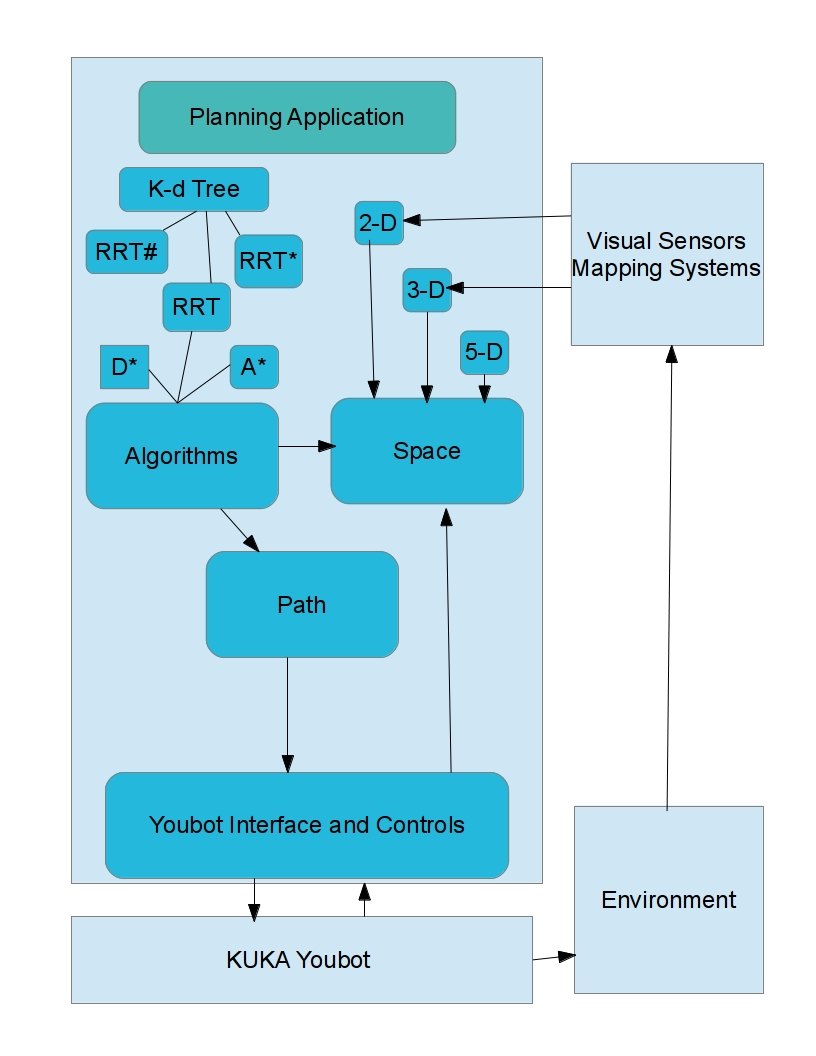
\includegraphics[width=90mm]{Simple Application Diagram.jpg}
\caption{This is a high-level simplified diagram of how the application we design will interact with the rest of the robot.}
\label{Planning Application}
\end{figure}

My idea for this semester project is the application shown in Figure 1. From the visual sensors we can determine a map of the area surrounding the robot. This map is two dimensional to determine where we want to move and three dimensional to determine the arms target. We also use information from the robot itself to determine the position of its joints(the 5-D space that the path planning algorithms will also have to handle) and the state of its actuators. Then, we run any of the assorted algorithms to output a path. Specifically, RRT's require a K-D tree for which I was unable to find a library last year which means we may need to implement it. The controller is then given the latest path information and then tries to follow it as closely as possible.

This rough diagram shows the growing complexity of the application in response to the difficult of the planning problem given to us. Ultimately, we are facing the challenges of transforming sensory information and our goals into actual commands.
\begin{thebibliography}{10}
\bibitem{RRT} \href{http://msl.cs.uiuc.edu/rrt/papers.html}{Rapidly-Exploring Random Trees}
\bibitem{RRTBidi} \href{http://people.csail.mit.edu/aperez/obirrt/}{Bidirectional RRTs}
\bibitem{RRTstar} \href{http://sertac.scripts.mit.edu/web/?page_id=15}{RRT*}
\bibitem{RRTsharp} \href{http://ieeexplore.ieee.org/xpl/login.jsp?tp=&arnumber=6630906&url=http://ieeexplore.ieee.org/iel7/6615630/6630547/06630906.pdf?arnumber=6630906}{RRT\#}
\bibitem{Astar} \href{http://dl.acm.org/citation.cfm?id=3830&coll=portal&dl=ACM}{A*}
\bibitem{Dstart} \href{http://citeseerx.ist.psu.edu/viewdoc/summary?doi=10.1.1.41.8257}{D*}
\bibitem{kdtree} \href{https://www.cise.ufl.edu/class/cot5520fa09/CG_RangeKDtrees.pdf}{K-D Trees}


\end{thebibliography}
\end{document}
